\documentclass{article}
\usepackage{fontspec}
\usepackage{xcolor}

\usepackage{amsthm}
\usepackage{amsmath}
\usepackage{amssymb}
\usepackage{unicode-math}
\usepackage[makeroom]{cancel}

\usepackage[normalem]{ulem}

\setmainfont{Times New Roman}
\setmathfont{Latin Modern Math}

\setlength\parindent{0em}
\setlength\parskip{0.618em}
\usepackage[a4paper,lmargin=1in,rmargin=1in,tmargin=1in,bmargin=1in]{geometry}

\usepackage{enumitem}

\usepackage{graphicx}

\usepackage{pgf,tikz,pgfplots}
\pgfplotsset{compat=1.15}
\usepackage{mathrsfs}
\usetikzlibrary{arrows}
\usetikzlibrary{plotmarks}



\begin{document}

\begin{center}
  $\mathcal{Dynamical\enskip Systems}$---$\mathcal{Final\enskip Exam}$

  \color{red}R\color{teal}icardo
  \color{red}J\color{cyan}.
  \color{red}A\color{teal}cu$\color{red}{\widetilde{\color{teal}\text{n}}}$\color{teal}a\color{black}

  \color{teal}(\color{red}862079740\color{teal})\color{black}
\end{center}
\vspace{1.618em}

\paragraph{1.}

\[\begin{cases}r^\prime = -r(2-r^2)(4-r)^3(6-r)\\
      \theta^\prime = 1\end{cases}\]

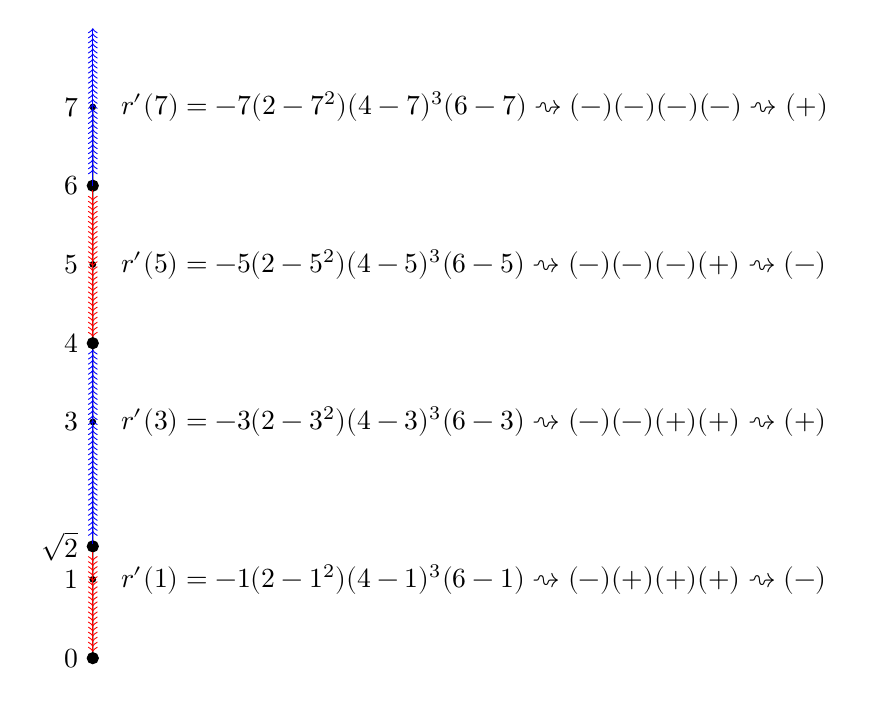
\begin{tikzpicture}
  \filldraw
                  (0,-1) circle (1pt)
                  node[align=left,  left,inner sep = 5pt] {$7$} --
                  (0,-1)
                  node[align=right,  right,inner sep = 10pt]
                  {$r^\prime(7) = -7(2-7^2)(4-7)^3(6-7)
                    \rightsquigarrow (-)(-)(-)(-)\rightsquigarrow (+)$} --
                  (0,-2) circle (2pt)
                  node[align=left, left,inner  sep = 5pt] {$6$}     --
                  (0,-3) circle (1pt)
                  node[align=left,  left,inner sep = 5pt] {$5$} --
                  (0,-3)
                  node[align=right,  right,inner sep = 10pt]
                  {$r^\prime(5) = -5(2-5^2)(4-5)^3(6-5)
                    \rightsquigarrow (-)(-)(-)(+)\rightsquigarrow (-)$} --
                  (0,-4) circle (2pt)
                  node[align=left, left,inner  sep = 5pt] {$4$}     --
                  (0,-5) circle (1pt)
                  node[align=left,  left,inner sep = 5pt] {$3$} --
                  (0,-5)
                  node[align=right,  right,inner sep = 10pt]
                  {$r^\prime(3) = -3(2-3^2)(4-3)^3(6-3)
                    \rightsquigarrow (-)(-)(+)(+)\rightsquigarrow (+)$} --
                  (0,-6.58) circle (2pt)
                  node[align=left, left,inner  sep = 5pt] {$\sqrt{2}$}     --
                  (0,-7) circle (1pt)
                  node[align=left,  left,inner sep = 5pt] {$1$} --
                  (0,-7)
                  node[align=right,  right,inner sep = 10pt]
                  {$r^\prime(1) = -1(2-1^2)(4-1)^3(6-1)
                    \rightsquigarrow (-)(+)(+)(+)\rightsquigarrow (-)$} --
                  (0,-8) circle (2pt)
                  node[align=left, left,inner  sep = 5pt] {$0$};
                  \draw[->>>>>>>>>>>>>>>>>>>>>>>>>>>>>>>>>>>>>,color=blue]
                  (0,-6.55) -- (0,-4.08);
                  \draw[->>>>>>>>>>>>>>>>>>>>>>>>>>>>>,color=blue]
                  (0,-2) -- (0,-0);
                  \draw[<<<<<<<<<<<<<<<<<<<-,color=red]
                  (0,-7.92) -- (0,-6.65);
                  \draw[<<<<<<<<<<<<<<<<<<<<<<<<<<<<-,color=red]
                  (0,-3.92) -- (0,-2.05);

\end{tikzpicture}

\[\begin{cases}r = \sqrt{x^2+y^2}\\
    \theta = \arccos\left(
      \frac{x}{\sqrt{x^2+y^2}}\right)\end{cases}\]

$\implies$

$r^\prime = \left(  \sqrt{x^2+y^2}\right)^\prime =
\frac{2xx^\prime+2yy^\prime}{2\sqrt{x^2+y^2}} =
\frac{2(xx^\prime+yy^\prime)}{2\sqrt{x^2+y^2}} = \frac{(xx^\prime+yy^\prime)}{\sqrt{x^2+y^2}} $

and

$\theta^\prime = \arccos\left(\frac{x}{\sqrt{x^2+y^2}}\right)^\prime$

$=
-\frac{1}{ \sqrt{1-\left(\frac{x}{\sqrt{x^2+y^2}}\right)^2}}\left(\frac{x}{\sqrt{x^2+y^2}}\right)^\prime$
$=-\frac{1}{
  \sqrt{1-\frac{x^2}{x^2+y^2}}}\left(\frac{x}{\sqrt{x^2+y^2}}\right)^\prime$
$= -\frac{1}{
  \sqrt{\frac{x^2+y^2-x^2}{x^2+y^2}}}\left(\frac{x}{\sqrt{x^2+y^2}}\right)^\prime$
$=
-\frac{1}{\frac{y}{\sqrt{x^2+y^2}}}\left(\frac{x}{\sqrt{x^2+y^2}}\right)^\prime$

$=
-\frac{\sqrt{x^2+y^2}}{y}\left(\frac{x}{\sqrt{x^2+y^2}}\right)^\prime$
$= -\left(\frac{\sqrt{x^2+y^2}}{y}\right) \frac{\sqrt{x^2+y^2}
  x^\prime - x (\sqrt{x^2+y^2})^\prime}{(\sqrt{x^2+y^2})^2}$
$= -\left(\frac{\sqrt{x^2+y^2}}{y}\right) \frac{\sqrt{x^2+y^2}
  x^\prime - x (\sqrt{x^2+y^2})^\prime}{x^2+y^2}$

$= -\frac{\frac{\sqrt{x^2+y^2}}{y} \sqrt{x^2+y^2} x^\prime -
  \frac{\sqrt{x^2+y^2}}{y} x (\sqrt{x^2+y^2})^\prime}{x^2+y^2}$
$= -\frac{\frac{\sqrt{x^2+y^2}}{y} \sqrt{x^2+y^2} x^\prime -
  \frac{\sqrt{x^2+y^2}}{y} x \frac{(xx^\prime+yy^\prime)}{\sqrt{x^2+y^2}}}{x^2+y^2}$
$= -\frac{x^\prime(x^2+y^2) - x (xx^\prime+yy^\prime)}{y(x^2+y^2)}$

$= -\frac{x^2x^\prime+y^2x^\prime -
  x^2x^\prime-xyy^\prime}{y(x^2+y^2)}$
$= -\frac{y^2x^\prime -xyy^\prime}{y(x^2+y^2)}$
$= -\frac{yx^\prime -xy^\prime}{x^2+y^2}$

$= \frac{xy^\prime -yx^\prime}{x^2+y^2}$

\newpage

Substitute with $r$ for convenience:

$r^\prime = \frac{(xx^\prime+yy^\prime)}{r}$ and $\theta^\prime =
\frac{xy^\prime -yx^\prime}{r^2}$

Substitute into the original polar system:

$\begin{cases}\frac{(xx^\prime+yy^\prime)}{r}
=
-r(2-r^2)
(4-r)^3(6-r)\\  \frac{xy^\prime -yx^\prime}{r^2} = 1\end{cases}$

$\frac{xy^\prime -yx^\prime}{r^2} = 1 \implies r^2 = xy^\prime -yx^\prime$


$\frac{(xx^\prime+yy^\prime)}{r} = -r(2-r^2)
(4-r)^3(6-r) \implies xx^\prime+yy^\prime = -r^2(2-r^2)
(4-r)^3(6-r)$

$r^2 = xy^\prime -yx^\prime$ $\implies xx^\prime+yy^\prime = -(xy^\prime -yx^\prime)(2-r^2)
(4-r)^3(6-r)$

$\implies xx^\prime+yy^\prime = yx^\prime(2-r^2)
(4-r)^3(6-r) -xy^\prime(2-r^2)
(4-r)^3(6-r)$

$\implies xx^\prime - yx^\prime(2-r^2)
(4-r)^3(6-r)= -yy^\prime -xy^\prime(2-r^2)
(4-r)^3(6-r)$

$\implies x^\prime(x - y(2-r^2)
(4-r)^3(6-r))= y^\prime(-y -x(2-r^2)
(4-r)^3(6-r))$

$\implies \frac{x^\prime }{y^\prime} =\frac{-y -x(2-r^2)
(4-r)^3(6-r)}{x - y(2-r^2)
(4-r)^3(6-r)}$


$\implies x^\prime =-y -x(2-r^2)
(4-r)^3(6-r)$
and
$ y^\prime = x - y(2-r^2)
(4-r)^3(6-r)$

Substitute $\sqrt{x^2+y^2}$ for $r$.

\[\begin{cases}
    x^\prime = -y -x(2-(x^2+y^2))
    (4-\sqrt{x^2+y^2})^3(6-\sqrt{x^2+y^2})\\
    y^\prime = x - y(2-(x^2+y^2))
    (4-\sqrt{x^2+y^2})^3(6-\sqrt{x^2+y^2})\end{cases}\]

Clearly, at $\begin{pmatrix} 0\\ 0 \end{pmatrix}$ there's an
equilibrium point. Furthermore, it is the only one. Going back to the
polar form, at $r=\sqrt{2}$ and $r=4$ and $r= 6$, $r^\prime =
0$. However, $\theta = 1$ no matter what happens to $r$. So, we get a
complete circle at each of those radii, as the angle is changing with
unit speed. Furthermore, they're limit cycles. One can see from the
phase portrait of the polar system, that the system satisfies the
properties (1),(2), and (3). Finally, for (4) the type of the origin is a
spiral sink. It can't be a regular sink, because if it were, $\theta^\prime$
would have to be $0$.

\paragraph{2.}

\[\begin{cases}
    x^\prime = bx + ay \\
    y^\prime = -x +by
\end{cases}\]

(1) $f(x,y) = bx + ay$ and $g(x,y) = -x +by$

A system is Hamiltonian $\iff$ $-f_x = g_y$.

$-f_x = -b$ and $g_y= b$

$-b = b \iff b = 0$

$\implies b = 0$ is the only value that makes this system Hamiltonian.

(2) Consider now the Hamiltonian system we get by letting $b = 0$ as a
one parameter family of ODEs.

\[(*)
  \begin{cases}
    x^\prime = ay \\
    y^\prime = -x
\end{cases}\]

Let $A = \begin{pmatrix}0&a\\-1&0\end{pmatrix}$ be the associated
matrix of $(*)$.

\newpage

Tr$(A) \equiv 0$, so $(*)$ is either a center or a saddle. As anything below trace-axis
is a saddle, and anything above is a center when the trace is $0$.

So, $|A| = 0$ $\implies 0^2-[(-1)\cdot a] = 0 \implies a = 0$ gives
the bifurcation point. Note, no other bifurcations can occur.

Let $a = 1:$  $\begin{pmatrix}0&1\\-1&0\end{pmatrix}$, the determinant
of this matrix is $1$, so it's a center.

$p(\lambda) = \lambda^2+1 = 0 \implies \lambda = \pm i$

$A_{1} - iI = \begin{pmatrix}-i&1\\-1&-i\end{pmatrix}
\stackrel{i\cdot R_2}{\rightarrow}
\begin{pmatrix} -i&1\\
  -i&-i^2\end{pmatrix}
=
\begin{pmatrix}
  -i&1\\
  -i&1
\end{pmatrix}
\stackrel{R_1- R_2}{\rightarrow}
\begin{pmatrix} -i&1\\
  0&0\end{pmatrix}
\stackrel{iR_1}{\rightarrow}
\begin{pmatrix} 1&i\\
  0&0\end{pmatrix}$

$\begin{pmatrix} 1&i\\
  0&0\end{pmatrix} \bold{v} = \begin{pmatrix} 1&i\\
  0&0\end{pmatrix} \begin{pmatrix}v_0\\ v_1\end{pmatrix}\implies
v_0 + v_1i=0  \implies v_0=-v_1i.$

Let $v_0=1 \implies v_1=i$

$\bold{v} = \begin{pmatrix}1\\ i\end{pmatrix} = \begin{pmatrix}1\\
  0\end{pmatrix} + i \begin{pmatrix}0\\ 1\end{pmatrix}$

$\implies \bold{x}(t) = e^{it}\bold{v} = \left[\cos(t)+i\sin(t)\right]\left[  \begin{pmatrix}1\\
    0\end{pmatrix} + i \begin{pmatrix}0\\ 1\end{pmatrix} \right]$

$ = \cos(t)\begin{pmatrix}1\\
  0\end{pmatrix} -\sin(t)\begin{pmatrix}0\\
  1\end{pmatrix} +i\left(\cos(t)\begin{pmatrix}0\\
  1\end{pmatrix} +\sin(t) \begin{pmatrix}1\\
  0\end{pmatrix}\right)$

$= \begin{pmatrix}\cos(t)\\
  -\sin(t)\end{pmatrix}+i \begin{pmatrix} \sin(t)\\
  \cos(t)\end{pmatrix} = \Re(t) +i\enskip \Im(t)$

$\implies \underbar{\overline{X}}(t) = \left[  \Re(t),\Im(t)\right] =
\begin{pmatrix}\cos(t)&\sin(t)\\
  -\sin(t)&\cos(t)\end{pmatrix} = R_{-t}$

Solutions are circles rotating clockwise.

Let $a = -1:$  $\begin{pmatrix}0&-1\\-1&0\end{pmatrix}$, the determinant
of this matrix is $-1$, so it's a saddle.

$p(\lambda) = \lambda^2-1 = 0 \implies \lambda = \pm 1$

$A_{-1} - I = \begin{pmatrix}-1&-1\\-1&-1\end{pmatrix}
\stackrel{R_1- R_2}{\rightarrow}
\begin{pmatrix} -1&-1\\
  0&0\end{pmatrix}
\stackrel{-1\cdot R_1}{\rightarrow}
\begin{pmatrix} 1&1\\
  0&0\end{pmatrix}$

$\begin{pmatrix} 1&1\\
  0&0\end{pmatrix}\bold{w} = 0
\implies \begin{pmatrix} 1&1\\
  0&0\end{pmatrix}\begin{pmatrix} w_0\\
  w_1\end{pmatrix} = 0 \implies w_0+w_1=0 \implies w_0 = -w_1$

Let $w_0 =1\implies w_1 = -1$

$\implies \bold{w} = \begin{pmatrix} 1\\
  -1\end{pmatrix}$

$A_{-1} + I = \begin{pmatrix}1&-1\\-1&1\end{pmatrix}
\stackrel{-1\cdot R_2}{\rightarrow}
\begin{pmatrix} 1&-1\\
  1&-1\end{pmatrix}
\stackrel{R_1- R_2}{\rightarrow}
\begin{pmatrix} 1&-1\\
  0&0\end{pmatrix}$

$\begin{pmatrix} 1&-1\\
  0&0\end{pmatrix}\bold{u} = 0
\implies \begin{pmatrix} 1&-1\\
  0&0\end{pmatrix}\begin{pmatrix} u_0\\
  u_1\end{pmatrix} = 0 \implies u_0-u_1=0 \implies u_0 = u_1$

Let $u_0 = u_1 = 1$
$\implies \bold{u} = \begin{pmatrix} 1\\
  1\end{pmatrix}$

$c_0\bold{w}+ c_1\bold{u} = 0 \implies c_0\begin{pmatrix} 1\\
  -1\end{pmatrix}+c_1\begin{pmatrix} 1\\
  1\end{pmatrix} = 0 \implies \begin{pmatrix} c_0+c_1\\
  -c_0+c_1\end{pmatrix} = 0 \implies c_0 +c_1= 0$ and $c_1-c_0 = 0$
$\implies c_0 = 0 = c_1$
$\implies \bold{w}$ and $\bold{u}$ are linearly independent.

$\implies \bold{x}(t) = e^t\bold{w}+e^{-t}\bold{u}$

$t\rightarrow \infty \implies \bold{x}(t) \rightarrow \bold{w}$
and
$t\rightarrow -\infty \implies \bold{x}(t) \rightarrow \bold{u}$

So, $\bold{w}$ is the future of $A_{-1}$ and $\bold{u}$ is it's past.

\paragraph{3.}

\[\begin{cases}
    x^\prime = 4y -4y^3 \\
    y^\prime = 2x -2
\end{cases}\]

(1)

Let $x^\prime = y^\prime = 0$ to find equilibria:


$\implies \begin{cases}
    0 = 4y -4y^3 = 4y(1-y^2) \\
    0 = 2x -2 = 2(x-1)
\end{cases}$
$\implies \begin{cases}
    0 = y(1 - y^2) \\
    x = 1
\end{cases}$

$\implies y = 0$ or $1-y^2 = 0$

$\implies y = \pm 1$

So, there are three equilibrium points
$\begin{pmatrix}1\\0\end{pmatrix}$, $\begin{pmatrix}1\\
  1\end{pmatrix}$, and $\begin{pmatrix}1\\ -1\end{pmatrix}$

The system is clearly Hamiltonian:

$f(x,y) = 4y -4y^3$ and $g(x,y) = 2x-2$

By inspection $-f_x = 0 = g_y$

In particular $f$ is a function of $y$, and $g$ is a function of $x$.

$\implies H(x,y) = \int 4y -4y^3 dy + \int 2x -2 dx = 4\int y -y^3 dy
+ 2\int (x -1) dx = 2y^2 -y^4 +x^2 -2x + C$

Let $C = 0: H(x,y) = 2y^2 -y^4 +x^2 -2x = y^2(2-y^2) -x(2-x)$

First, determine what happens at the equilibria---i.e: the trivial
cycles.

$H(1, 0)= (0)^2(2-(0)^2) -1(2-1) = -1(2-1) = -1$

Consider $H^{-1}(-1) = \{(x,y)\in \BbbR| y^2(2-y^2) -x(2-x) = -1\}$

$\implies y^2(2-y^2) -x(2 -x) = -1$

$\implies y^2(2-y^2) +1 -x(2-x) = 0$

$\implies -y^4+ 2y^2 +1 +x^2 -2x = 0$

$\implies y^4 - 2y^2 -1 -x^2+ 2x = 0$

$\implies y^2 = \frac{2 \pm \sqrt{4 -4\cdot(1)(-1 -x^2+ 2x)}}{2} = 1
\pm \frac{2\sqrt{1 -(-1 -x^2+ 2x)}}{2}  = 1 \pm \sqrt{1 +1 +x^2- 2x} = 1
\pm \sqrt{x^2-2x + 2}$

$\implies y = \pm \sqrt{1
\pm \sqrt{x^2-2x+2}}$

$y$ is only defined, when $1
\pm \sqrt{x^2-2x+2} > 0$ and $x^2-2x+2 > 0$

$1 \pm \sqrt{x^2-2x+2} = 0$ $\implies \pm \sqrt{x^2-2x+2} = -1$

$\implies x^2-2x+2 = 1$ $\implies x^2-2x+1 = 0$

$\implies x = \frac{2\pm \sqrt{4-4}}{2} = 1$, which we already knew.

$\implies x^2-2x +2 = 0 \implies x = \frac{2\pm \sqrt{4-8}}{2} = 1\pm
i$, which tells us $\sqrt{x^2-2x+2}$ is defined everywhere.

In particular $\sqrt{1^2-2(1)+2} = 1$, so since as a function it has
no $x$-intercept $\sqrt{x^2-2x+2} > 0$ for all $x \in \BbbR$.

So, $1 + \sqrt{x^2-2x+2} > 0$ for all $x \in \BbbR$. So, $y$ is well
defined when $y = \pm\sqrt{1 + \sqrt{x^2-2x+2}}$.


Want to show $1 -\sqrt{x^2-2x+2} \leq 0$

Assume $1 -\sqrt{x^2-2x+2} > 0$, then $-1 +\sqrt{x^2-2x+2} < 0$

$\implies \sqrt{x^2-2x+2} < 1$ $\implies x^2-2x+2 < 1$ $\implies
x^2-2x +1 < 0 \implies (x-1)^2 < 0$ is false.

So, by contradiction $1 -\sqrt{x^2-2x+2} \leq 0$.



So, the only real solution of $y = \pm \sqrt{1
- \sqrt{x^2-2x+2}}$, is $x = 1$. Therefore, we can drop the $\pm$ in
that case. So, $y = \sqrt{1
  - \sqrt{x^2-2x+2}} \implies y = 0$ and $x = 1$.

\newpage

For $x = 1$ in $y = \pm \sqrt{1
  + \sqrt{x^2-2x + 2}}$

$y = \pm \sqrt{1
  + \sqrt{1^2-2(1)+2}} = \pm  \sqrt{2}$


Considering half of the trajectories:

$y^\prime = \frac{\frac{2x-2}{2\sqrt{x^2-2x+2}}}{2\sqrt{1
    + \sqrt{x^2-2x+2}}} = \frac{\frac{x-1}{\sqrt{x^2-2x+2}}}{2\sqrt{1
    + \sqrt{x^2-2x+2}}} = \frac{x-1}{2\sqrt{1
    + \sqrt{x^2-2x+2}}\sqrt{x^2-2x+2}} = 0$

Both $2\sqrt{1
  + \sqrt{x^2-2x+2}}$ and $\sqrt{x^2-2x+2}$ are bigger than $0$,

so $\frac{x-1}{2\sqrt{1
    + \sqrt{x^2-2x+2}}\sqrt{x^2-2x+2}} = 0$

$ \implies x-1=0 \implies x =
1$

$x = 1$ is a critical point.

Now,

$y^{\prime\prime} = \frac{2\sqrt{1
    + \sqrt{x^2-2x+2}}\sqrt{x^2-2x+2} -(x-1)\left( 2\sqrt{1
      + \sqrt{x^2-2x+2}}\sqrt{x^2-2x+2}\right)^\prime}{4(1
  + \sqrt{x^2-2x+2})(x^2-2x+2)}$


Compute $\left( 2\sqrt{1
    + \sqrt{x^2-2x+2}}\sqrt{x^2-2x+2}\right)^\prime $

$= 2 \left(\sqrt{1
    + \sqrt{x^2-2x+2}}\sqrt{x^2-2x+2}\right)^\prime $

$= 2\left[  \left(\sqrt{1
      + \sqrt{x^2-2x+2}}\right)^\prime \sqrt{x^2-2x+2} +\sqrt{1
    + \sqrt{x^2-2x+2}} \left(\sqrt{x^2-2x+2}\right)^\prime\right]$

$= 2\left[\frac{x-1}{2\sqrt{1
    + \sqrt{x^2-2x+2}}\sqrt{x^2-2x+2}}
 \sqrt{x^2-2x+2} +\sqrt{1
   + \sqrt{x^2-2x+2}} \frac{2x-2}{2\sqrt{x^2-2x+2}}\right]$

$= 2\left[\frac{x-1}{2\sqrt{1
    + \sqrt{x^2-2x+2}}} +\sqrt{1
   + \sqrt{x^2-2x+2}} \frac{x-1}{\sqrt{x^2-2x+2}}\right]$


$= 2(x-1)\left[\frac{1}{2\sqrt{1
    + \sqrt{x^2-2x+2}}} +\sqrt{1
  + \sqrt{x^2-2x+2}} \frac{1}{\sqrt{x^2-2x+2}}\right]$

$y^{\prime\prime} = \frac{2\sqrt{1
    + \sqrt{x^2-2x+2}}\sqrt{x^2-2x+2} -(x-1)2(x-1)\left[\frac{1}{2\sqrt{1
    + \sqrt{x^2-2x+2}}} +\sqrt{1
  + \sqrt{x^2-2x+2}} \frac{1}{\sqrt{x^2-2x+2}}\right]}{4(1
+ \sqrt{x^2-2x+2})(x^2-2x+2)}$


$y^{\prime\prime}(1) = \frac{2\sqrt{2} -(1-1)2(x-1)\left[\frac{1}{2\sqrt{1
    + \sqrt{x^2-2x+2}}} +\sqrt{1
  + \sqrt{x^2-2x+2}} \frac{1}{\sqrt{x^2-2x+2}}\right]}{4(1
+ \sqrt{x^2-2x+2})(x^2-2x+2)} = \frac{2\sqrt{2}}{4(2)} =
\frac{\sqrt{2}}{4} > 0$

By the second derivative test at $x = 1$, $y$ is concave up. So, $x =
1$ is a local minimum of $y$. Similarly, the negative
trajectory has a local maximum at $x = 1$, because their first and
second derivatives differ by a sign.

So, there cannot be any homoclinic trajectory in this case. $y = \pm \sqrt{1
  + \sqrt{x^2-2x + 2}}$, is either positive or negative always. $y = \pm \sqrt{1
  - \sqrt{x^2-2x + 2}}$ is actually only one point $x=1$ and $y =0$.

$H(1,\pm 1)= (\pm 1)^2(2-(\pm 1)^2) -1(2-1) = 1(2-1)-1(2-1) = 0$

$H^{-1}(0) = \{(x,y) \in \BbbR | y^2(2-y^2) -x(2-x) = 0\}$:

$H(x,y) = y^2(2-y^2) -x(2-x) = 0 $

$\implies -y^4+2y^2 -x(2-x) = 0$

$\implies y^4-2y^2 +x(2-x) = 0$

$\implies y^2 = \frac{2 \pm \sqrt{4-4x(2-x)}}{2} = 1 \pm
\sqrt{1-x(2-x)} = 1 \pm
\sqrt{x^2-2x +1)} = 1 \pm \sqrt{(x-1)^2} = 1 \pm (x-1) $

$\implies y = \pm \sqrt{1 \pm (x-1)}$

$y$ is defined only when  $1 \pm (x-1) \geq 0$:

$1 + (x-1) \geq 0 \implies x \geq 0$

So, the $x$-intercept of $y = \pm \sqrt{1 + (x-1)}$ is $x = 0$

$1 - (x-1) \geq 0 \implies 1 -x + 1 \geq 0 \implies 2 \geq x$

So, the $x$-intercept of $y = \pm \sqrt{1 - (x-1)}$ is $x = 2$

Therefore, in between
$\begin{pmatrix}1\\ \pm 1\end{pmatrix}$ are two
heteroclinic orbits passing through
$\begin{pmatrix}0\\
  0\end{pmatrix}$ in the case of $y = \pm \sqrt{1 + (x-1)}$, and $\begin{pmatrix}2\\
  0\end{pmatrix}$ in the case of $y = \pm \sqrt{1 - (x-1)}$

Since, I classified all the equilibrium points, I conclude there are
no heteroclinic orbits.

(2) Since, there's no homoclinic trajectory I'll interpret the
question as classify all trajectories.

I've shown that there's only one trivial cycle at $\begin{pmatrix}1\\
  0\end{pmatrix}$. Together with the two equilibria $\begin{pmatrix}1\\
  \pm 1\end{pmatrix}$ and the 6
heteroclinic trajectories connecting them, I've only shown 2, the ones
passing through $\begin{pmatrix}0\\
  0\end{pmatrix}$ and $\begin{pmatrix}2\\
  0\end{pmatrix}$, however since $y$ and $-y$ are continuous and everywhere
defined there must be 2 trajectories above $\begin{pmatrix}1\\
  1\end{pmatrix}$, and 2 below $\begin{pmatrix}1\\
  -1\end{pmatrix}$.

Now, given that the system is Hamiltonian $\forall C \in \BbbR,$ each $H^{-1}(C)$ is
and bounded, closed, invariant set. $\forall C:$ If $C$ is not $-1$ or
$0$, then $H^{-1}(C)$ does not contain any equilibrium points. So,
from Corollary 2 of Poicaré-Bendixon Theorem, It follows that
$H^{-1}(C)$ only contains cycles. And, it sounds silly that I'm
repeating it for a third time $H^{-1}(0)$, contains only $\begin{pmatrix}1\\
  0\end{pmatrix}$ so it's a trivial cycle.

\newpage
\paragraph{4.}

\[\begin{cases}
x^\prime = 3x -x^2 -xy\\
y^\prime = 2y -y^2 -\frac{1}{2}xy
\end{cases}\]

(1) Well, this clearly is a competitive species model, since we have
$-b xy$, in each rate of change. However it's funny because, we have a
$-x^2$ term in $x^\prime$, and a $-y^2$ term in $y^\prime$. It's funny
because it means that each species is competing with itself for
resources. I think it's a more natural model however. We as humans do
precisely that. We're constantly competing for resources with
each other, not only as individuals, but as families, and even as nations.

Now let's do some analysis on this.

Let $x^\prime = y^\prime = 0$

\[\begin{cases}
0 = 3x -x^2 -xy\\
0 = 2y -y^2 -\frac{1}{2}xy
\end{cases}\]

$\implies 3x -x^2 -xy = 0 \stackrel{\cdot -1}{\implies}
x^2 -3x + xy = x^2 + (y-3)x=0$

$\implies x= \frac{-(y-3)\pm \sqrt{(y-3)^2-4\cdot 1\cdot 0}}{2}
=\frac{-(y-3)\pm(y-3)}{2}$

$\implies x = 0$ or $x = \frac{-(y-3)-(y-3)}{2} =\frac{-2(y-3)}{2} =
-(y-3) = 3-y$

$\implies x = 3 -y $ $\guillemotright a \guillemotleft$

If $x = 0$, then $0 = 2y -y^2 -\frac{1}{2}0y$

$\implies 0 = 2y - y^2 =
y(2-y) \implies y = 0$  or $y = 2$

If $x = 3-y$, then $0 = 2y -y^2 -\frac{1}{2}(3-y)y $

$\implies 0 = 2y -y^2 -\frac{3}{2}y+ \frac{1}{2}y^2 = -\frac{1}{2}y^2
+\frac{1}{2}y$

$\stackrel{\cdot -2}{\implies} 0= y^2 - y = y(1-y)$

$\implies y = 0$ or $y = 1$

So if $y = 0$, then $x = 3-0 =3$. And if $y = 1$, then $x = 3 -1 = 2$.

Therefore all the equilibria are, $\begin{pmatrix} 0\\0\end{pmatrix}$,
$\begin{pmatrix} 0\\2\end{pmatrix}$, $\begin{pmatrix}
  3\\0\end{pmatrix}$, and $\begin{pmatrix} 2\\1\end{pmatrix}$.

(2) So, yes two species can coexist with each other, $\begin{pmatrix}
  2\\1\end{pmatrix}$ is an equilibrium solution of the system, where
neither $x$, nor $y$ are $0$.

(3)

The $v$-nullclines I already determined from $\guillemotright a
\guillemotleft$ to satisfy $x = 3 -y$

$\implies y = -x + 3$

Two points on the $v$-nullcline are, $\begin{pmatrix} 3\\0\end{pmatrix}$ and $\begin{pmatrix} 0\\3\end{pmatrix}$.

For the $h$-nullclines analize  $0 = 2y -y^2 -\frac{1}{2}xy $

$\implies $ $0 = y(2 -y -\frac{1}{2}x)$

$\implies y = 0$ or $0 = 2 -y -\frac{1}{2}x$

$\implies y = -\frac{1}{2}x + 2$

Two points on the $h$-nullcline are, $\begin{pmatrix}
  4\\0\end{pmatrix}$ and $\begin{pmatrix} 0\\2\end{pmatrix}$.

$-x + 3 = -\frac{1}{2}x + 2 \implies \frac{1}{2}x =1 \implies x = 2$
and $y = 3-2 = 1$

Now, if $y \equiv 0$. This reduces to the following one dimensional system:

\[\begin{cases}
x^\prime = 3x -x^2 = x(3-x)\\
y^\prime \equiv 0
\end{cases}\]

$x^\prime(4) = 4(3-4)
\rightsquigarrow (+)(-)\rightsquigarrow (-)$
and
$x^\prime(1) = 1(3-1)
    \rightsquigarrow (+)(+)\rightsquigarrow (+)$

Similarly for $x \equiv 0$:

\[\begin{cases}
x^\prime \equiv 0\\
y^\prime = 2y -y^2 = y(2-y)
\end{cases}\]


$y^\prime(4) = 4(2-4)\rightsquigarrow (+)(-)\rightsquigarrow (-)$

and

$y^\prime(1) = 1(3-1)
    \rightsquigarrow (+)(+)\rightsquigarrow (+)$

Combining all that information I get the following phase portrait:

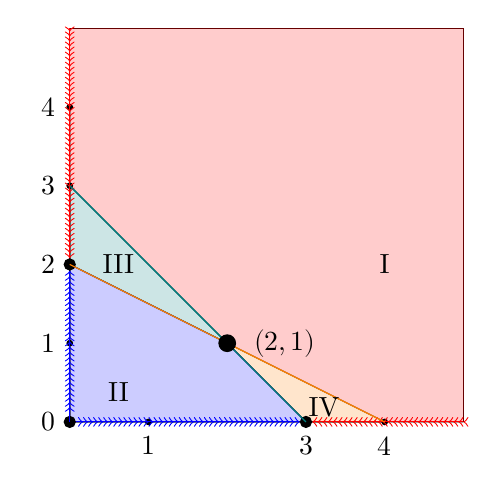
\begin{tikzpicture}
  \filldraw[fill=red!20!white, draw=red!40!black]
  (0,1) rectangle(5,-4);
  \filldraw[fill=orange!20!white, draw=orange!40!black]
  (3,-4) -- (4,-4) -- (2,-3) -- cycle;
  \filldraw[fill=teal!20!white, draw=teal!40!black]
  (0,-1) -- (0,-2) -- (2,-3) -- cycle;
  \filldraw[fill=blue!20!white, draw=blue!40!black]
  (0,-4) -- (0,-2) -- (2,-3) -- (3,-4) -- cycle;
  \filldraw
  (5,-4) --
  (4,-4) circle (1pt)
  node[align=left,  below,inner sep = 5pt] {$4$} --
  (3,-4) circle (2pt)
  node[align=left, below,inner  sep = 5pt] {$3$} --
  (1,-4) circle (1pt)
  node[align=left,  below,inner sep = 5pt] {$1$} --
  (0,-4);

  \draw[->>>>>>>>>>>>>>>>>>>>>>>>>>>>>>>>>>>>>>>>>>>>,color=blue]
  (0,-4) -- (2.92,-4);
  \draw[<<<<<<<<<<<<<<<<<<<<<<<<<<<<<<<-,color=red]
  (3.08,-4) -- (5,-4);


  \filldraw
  (0,0) circle (1pt)
  node[align=left,  left,inner sep = 5pt] {$4$} --
  (0,-1) circle (1pt)
  node[align=left, left,inner  sep = 5pt] {$3$} --
  (0,-2) circle (2pt)
  node[align=left, left,inner  sep = 5pt] {$2$}     --
  (0,-3) circle (1pt)
  node[align=left,  left,inner sep = 5pt] {$1$} --
  (0,-4) circle (2pt)
  node[align=left, left,inner  sep = 5pt] {$0$};

  \draw[->>>>>>>>>>>>>>>>>>>>>>>>>>>>,color=blue]
  (0,-4) -- (0,-2.08);
  \draw[<<<<<<<<<<<<<<<<<<<<<<<<<<<<<<<<<<<<<<<<<<<<<<-,color=red]
  (0,-1.92) -- (0,1);

  \draw[orange]
  (4,-4) --
  (0,-2);

  \draw[teal]
  (3,-4) --
  (0,-1);

  \filldraw
  (2,-3) circle (3pt);
  \node[right=0.618em] at (2,-3) {$(2,1)$};

  \node at (4,-2) {I};
  \node at (0.618,-3.618) {II};
  \node at (0.618,-2) {III};
  \node at (3.23,-3.82) {IV};

\end{tikzpicture}

In green, we have the $v$-nullcline. And, in orange we have the
$h$-nullclines. They meet at $\begin{pmatrix}
  2\\1\end{pmatrix}$, which is one of the equilibrium points we found
before. Region I, is a positively invariant set, it encloses regions II,III,
and IV---i.e: all point's not all ready in I will eventually enter
I. Both, II, III are positively invariant sets, from the direction of
the $h$-nullclines and $v$-nullclines. And, IV is negatively
invariant---i.e: Nothing can enter IV, but everything comes from IV. $\begin{pmatrix}
  0\\0\end{pmatrix}$ is a source, $\begin{pmatrix}
  3\\0\end{pmatrix}$, and $\begin{pmatrix}
  0\\2\end{pmatrix}$ are saddles, and $\begin{pmatrix}
  2\\1\end{pmatrix}$ is a global sink.

(4)

It's clear from the picture that $\begin{pmatrix}
  0\\0\end{pmatrix}$
is a source. So, I can
apply Corollary 5 of the Poicaré-Bendixon Theorem. The ODE system in question is
nice so we have Existence and Uniqueness of solutions, so it defines a dynamical
sytem $\Phi$.

Actually, I need to apply the contrapositive of Corollary 5. Corollary
5 reads: Let $\Phi$ be a planar system that has a first integral which
is non-constant on any open ball, then $\Phi$ may not have a sink, a
source, or a limit cycle.

The contrapositive reads: If $\Phi$ has a sink, a
source, or a limit cycle, then $\Phi$ doesn't have a first integral which
is non-constant on any open ball.

$\Phi$ has a sink, so any first integral must be constant on any open
ball---i.e any first integral of $\Phi$ must be trivial.

\paragraph{5.} My favorite part of the course was the idea that we can
actually get very valuable information out of systems of differential
equations that are not solvable. For instance, the fact that there
doesn't exist a nontrivial first integral to the previous problem
would've stopped a lot of analysis from ever happening. Now, I have
tools to solve seemingly intractable problems.



\end{document}

%%% Local Variables:
%%% mode: latex
%%% TeX-master: t
%%% End:
